\documentclass{standalone}
\usepackage{ tikz }
\usetikzlibrary{shapes}
\usetikzlibrary{plotmarks}
\usepackage{ xparse }
\usepackage{../../../macros}

\begin{document}
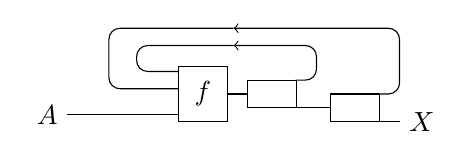
\begin{tikzpicture}[yscale=-1,x=1em,y=1.25em]
        
    \node [anchor=east] at (0.5,0) {$A$};
    \draw (0.5,0) -- (4.5,0);
    \draw (3.75,-0.75) -- (4.5,-0.75);
    \node[draw, minimum height = 2em, minimum width = 1.75em, anchor = west] at (4.5,-0.6){$f$};
    \draw (6.25,-0.6) -- (7,-0.6);
    \node[draw, minimum height = 1em, minimum width = 1.75em, anchor = west] at (7,-0.6){$\ccopy{}$};
    \draw [rounded corners,->] (8.75, -1) -- (9.5, -1) -- (9.5,-2) -- (6.5,-2);
    \draw [rounded corners] (6.5,-2) -- (3,-2) -- (3,-1.25) -- (4.5,-1.25);
    \draw (8.75,-0.2) -- (10,-0.2);
    \node[draw, minimum height = 1em, minimum width = 1.75em, anchor = west] at (10,-0.2){$\ccopy{}$};
    \draw [rounded corners, ->] (11.75,-0.6) -- (12.5,-0.6) -- (12.5,-2.5) -- (6.5, -2.5);
    \draw [rounded corners] (6.5,-2.5) -- (2, -2.5) -- (2,-0.75) -- (4.5,-0.75);
    \draw (11.75, 0.2) -- (12.5,0.2);
    \node [anchor=west] at (12.5,0.2) {$X$};
\end{tikzpicture}
\end{document}